

%\vspace*{-20mm}
% \centerline{\underline{\Large\bf Атомная физика}}\vspace{5mm}

\centerline{\large\bf Проблема: у света $\exists$ корпускулярные свойства
 (а не только волновые!)}
\begin{itemize}
\item Если считать суммарную мощность излучения абсолютно черного тела по классической электродинамике (Рэлей \& Джинс), то получается {\bf абсурдный} результат ($W x\rightarrow\infty$). Но все становится разумным, если верна непонятная гипотеза {\bf Макса Планка} о том, что излучение не непрерывно, а возможно лишь порциями $\varepsilon=h\nu$, где $h=6.624\cdot10^{-27}$ эрг (постоянная Планка), а $\nu$ -частота излучения.
\item В рентгеновском спектре $\exists$ {\bf левая граница} ($\lambda\geq\lambda_{min}$), зависящая от напряжения питания рентгеновской трубки U: $\lambda_{\rm min}$[{\AA}]=12350/U[V]. То есть, вроде как и в самом деле один электрон с $E=eU$ не может породить фотон с $h\nu=\varepsilon>E$.
\item {\bf Фотоэффект}: ток не зависит от напряжения ($\exists$ насыщение), но пропорционален ин\-тен\-сив\-но\-с\-ти облучения светом; тока нет совсем, если $\lambda\geq\lambda_{\rm min}$ (то есть, если энергия одного фотона < работы выхода электрона из облучаемого металла). При уменьшении $\lambda$ энегрия выбитых электронов растет линейно с частотой света. Кроме того, фотоэлектроны появляются {\bf сразу} после начала облучения (даже если свет ОЧЕНЬ слабый) --  то есть, нет ``накопления'' энергии слабой волны до порогового значения.
\end{itemize}
{\bf Альберт Эйншнейн}: не только излучение, но и поглощение света идет {\bf КВАНТАМИ}.
Вывод: свет -- это ФОТОНЫ (=кванты электромагнитного излучения). Свойства -?

\begin{itemize}
\item Энергия фотона: $\varepsilon=h\nu$\\
 \begin{tabular}{lrcc}
 ИК:  & $\lambda=10\mu m$ & $\varepsilon=2\cdot 10^{-13}$ эрг & $\simeq 0.1$ эВ\\
 видимый свет:  &$\lambda$=5000{\AA} & $\varepsilon=4\cdot10^{-12}$ эрг & $\simeq 2.5$ эВ\\
 X-лучи:  &$\lambda$=0.1 {\AA} & $\varepsilon=2\cdot10^{-7}$ эрг & $\simeq 70$ кэВ\\
 \end{tabular}\\
 Корпускулярные св-ва проявляются сильнее при больших энергиях (малых $\lambda$)
\item Масса фотона =0 (т.к. фотон {\sl по определению} движется со скоростью света, а энергия не $\infty$, то его масса по законам релятивистской механики просто обязана быть $\equiv$ 0).
\item Количество движения (импульс) фотона связан с его энергией:
\begin{displaymath}
E^2=\left(mc^2\right)^2+(pc)^2\hspace{20mm}(m=0)\Rightarrow\hspace{10mm}E=pc\hspace{10mm}\Rightarrow\hspace{10mm}
p=\frac{h\nu}c
\end{displaymath}
И действительно, известно ``световое давление''!
\item {\bf Артур Комптон} (1923): рассеяние Х-лучей. Среди рассеянных $\exists$ лучи не только с $\lambda=\lambda_0$, но и с $\lambda>\lambda_0$!!! \\
    Объяснение: до рассеяния был фотон с энергией $h\nu_1$ и импульсом $\vec{p}_\gamma$ + покоящийся $e^-$. После рассеяния $e^-$ приобрел отдачу (энергию $E_e$ и импульс $\vec{p}_e$), а фотон ЭТО ЖЕ потерял: $h\nu_2 = h\nu_1 - E_e$, \hspace{10mm} $\vec{p}_2=\vec{p}_1-\vec{p}_e$. Если все аккуратно посчитать, то можно получить известную формулу:
\begin{displaymath}
E_1-E_2=\frac{E_1E_2}{mc^2}\;(1-\cos\varphi)\hspace{20mm}\texttt{или}\hspace{20mm}
 \lambda_2-\lambda_1=\frac{hc}{mc^2}\;(1-\cos\varphi)
\end{displaymath}
где $\varphi$ -- угол рассеяния фотона.
\end{itemize}
Но и волновые свойства света никто не отменял (интерференция, дифракция, поляризация, отражение, преломление)...\\
Накопилось много фактов, толкающих к созданию новой (не классической) физики, которая бы все это как-то объясняла.\\

%\newpage
\section{Проблемы со строением атома}
%\centerline{\Large\bf Проблемы со строением атома.}

\begin{picture}(190,50)(0,0)
\put(50,0){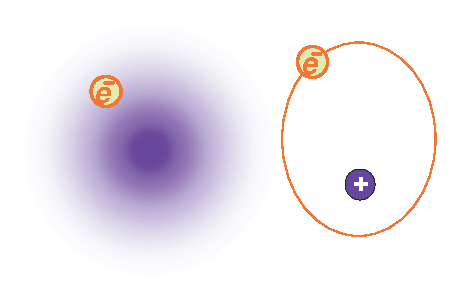
\includegraphics{GP028/GP028F01.eps}}
 \put( 50,45){\makebox(0,0)[lt]{\bf Модель Томсона}}
 \put(90,45){\makebox(0,0)[lt]{\bf Модель Резерфорда}}
 \put(0,38){\makebox(0,0)[lt]{\parbox{52mm}{
 Атом -- это равномерно (или почти равномерно) положительно заряженный шарик, и в нем мечутся точечные отрицательные электроны).
 }}}
 \put(180,38){\makebox(0,0)[rt]{\parbox{57mm}{
 Атом -- это положительно заряженное точечное мас\-сив\-ное ядро, и вокруг него (как планеты вокруг Солнца) летают точечные отрицательные электроны).
 }}}
\end{picture}\\[5mm]
Первая модель: почему заряженный рыхлый шарик не разваливается? Если он не рыхлый -- то как электрон через него проникает? \\
Вторая модель лучше. Но непонятно: почему движущийся электрон не излучает и почему он не падает на ядро?\\
Опыт Резерфорда по рассеянию $\alpha$-частиц: если бы шарик был рыхлым, то не было бы рассеяния на большие углы (а оно бывает). Вывод: ядро есть! Но почему же нет излучения?...\\[10mm]
%\vspace*{5mm}

\section{Проблемы с оптическими спектрами}
%\centerline{\Large\bf Проблемы с оптическими спектрами.}\\[3mm]

{\bf Бальмер} (Базель, 1885): в линейчатых спектрах испускания $\exists$ какая-то странная закономерность.\\
\begin{picture}(190,30)(0,0)
\put(10,0){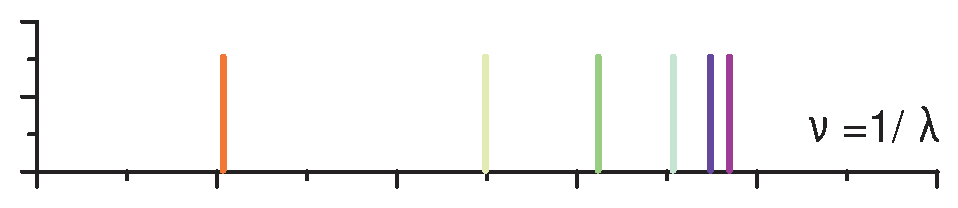
\includegraphics{GP028/GP028F02.eps}}
\end{picture}\\[5mm]
\begin{displaymath}
\lambda_n=\lambda_0\cdot\frac{n^2}{n^2-4}
\end{displaymath}
где $n$ -- некоторое целое число: $n$=3, 4, 5, ...

В спектроскопии традиционно вместо обычной частоты принято использовать волновое число $\nu$ (сколько $\lambda$ уместится в 1 см):
\begin{displaymath}
\nu\equiv\frac{1 \texttt{см}}\lambda \hspace{10mm}[\nu]={cm}^{-1}.
\end{displaymath}
Так вот, у Бальмера получилось, что для многих атомов $\nu=A-R/n^2$.

Позднее {\bf Ридберг} (Лунд, Швеция, 1888) определил, что $A=R/4$ (выполняется очень точно!), и тогда можно сказать, что
\begin{displaymath}
 \nu =R\cdot\left(\frac1{2^2}-\frac1{n^2}\right)\hspace{20mm}R=109737.316\;\; {cm}^{-1}
\end{displaymath}
(потом эту константу $R$ назвали постоянной Ридберга).

Получалось, что есть какие-то ТЕРМЫ (наподобие энергетических уровней), и излучение -- это комбинация РАЗНОСТЕЙ между термами. Для них даже придумали названия: 1S, 2P, 3P, 4D, и т.д.

В это время {\bf Нильс Бор} (Копенгаген, 1913) как раз думал об устройстве атома. {\em ``Как только я увидел формулу Бальмера, весь вопрос стал мне немедленно ясен.'' }

\section{Атом, который построил Бор}
%{\Large \bf Атом, который построил Бор}

Есть {\bf дискретные стационарные} состояния атома. Находясь в них, атом ничего не излучает. Излучение возникает (или поглощается) только при переходе между состояниями. Что это за состояния? Бор: стационарными являются лишь те, для которых угловой момент количества движения ($\mathcal{L}=pr=\mathcal{I}\omega=m\cdot v\cdot r$)
кратен целому числу:
\begin{displaymath}
\mathcal{L}=n\cdot\hbar=n\cdot\frac{h}{2\pi}\hspace{20mm}\left(\hbar=\frac{h}{2\pi}\right)
\end{displaymath}
Если считать, что электрон крутится по круговой орбите с радиусом $r$ и удерживается на ней кулоновской силой, то:
\begin{displaymath}
\texttt{(центростремительная сила:) }
\frac{mv^2}r =\frac{Ze^2}{r^2}
\texttt{ (- кулоновскаяая сила)}
\end{displaymath}
учтем, что по Бору $mvr=n\hbar$,  избавимся от $v$ и затем найдем $r$:
\begin{displaymath}
v=\frac{n\hbar}{mr}\hspace{20mm} \frac{mn^2\hbar^2}{m^2r} =Ze^2\hspace{20mm}r=\frac{n^2\hbar^2}{Zme^2}
\end{displaymath}
Если теперь вычислить первый боровский радиус $a_0$ (то есть, положить $Z$=1 и $n$=1), то получим нечто очень похожее на правду:
\begin{displaymath}
a_0=\frac{\hbar^2}{me^2}=0.529\;\;{\texttt{\AA}}
\end{displaymath}
Полная энергия =
\begin{displaymath}
W_p+W_k=-\frac{Ze^2}{r}+\frac{mv^2}2=-\frac{Ze^2}{r}+\frac{Ze^2}{2r}=-\frac{Ze^2}{2r}=
-\frac{Ze^2\;Zme^2}{2\;n^2\hbar^2}=-\frac{mZ^2e^4}{2\hbar^2n^2}
\end{displaymath}
При переходе с $n_1$ на $n_2$ частота будет
\begin{displaymath}
\nu=\frac{\varepsilon}{h}=\frac{W_1-W_2}{h}=\frac{mZ^2e^4}{4\pi\hbar^3}\cdot\left(\frac1{n_1^2}-\frac1{n_2^2}\right)
\end{displaymath}
и, следовательно, в серии Бальмера были переходы с $n_1$=3,4,5,.. на $n_2$=2. Значит, должны еще где-то быть и другие серии, например: $n_1$=2,3,4,5,.. на $n_2$=1.  После такого предсказания Бора Лайман действительно нашел эту серию (просто она в УФ-диапазоне была, поэтому ее раньше не заметили).

Если еще учесть, что не только электрон движется, но и ядро, то получается совсем хорошо: даже видна разница между протием и дейтерием (в 4-ом знаке отличие). Короче, после Бора в оптике наступила эйфория. Непонятно только было, ПОЧЕМУ так все хитро устроено? \\[5mm]
{\bf Луи де Бройль} (Louis-Victor-Pierre-Raymond, 7\`{e}me duc de Broglie, Дьепп, 1924):  Может, не только у света есть корпускулярные свойства, но и у всех частиц -- волновые?...  Если мы фотону с длиной волны $\lambda$ (или частотой $\nu$) сопоставляем энергию $\varepsilon=h\nu$ и импульс $p=h\nu/c=h/\lambda$, то почему бы {\em``нормальной''} частице, имеющей энергию $\varepsilon$ и импульс $p=mv$ не сопоставить какую-то волну с длиной $\lambda=h/p$? (Поскольку $\varepsilon=h\nu=h/T=hc/\lambda$, а $p=\varepsilon/c=h/\lambda$)

Когда через 3 года экспериментально была обнаружена дифракция электронов на кристалле, за эту дерзкую мысль Луи де Бройлю была вручена Нобелевская премия.

Например, при $E_e=1$ кэВ дебройлевская длина волны электрона $\lambda=h/mv=h/\sqrt{2mE}\simeq0.4${\AA}, то есть, схожа с рентгеном. Поскольку электроны легко можно разогнать до МэВ, то $\lambda$ будет еще короче, и, следовательно, можно сделать электронный микроскоп, способный различать совсем малые объекты (в 1000 раз меньше, чем оптический).

Каков физический смысл такой как бы волны? Чтобы не путать с другими (настоящими) волнами, ее называют волновой функцией, зависящей от координат и времени: $\Psi(x,y,z,t)$. Если поле, в котором частица движется, стационарно (а мы до других случаев в этом курсе не дойдем), то можно ее представить в виде двух сомножителей:
\begin{displaymath}
\Psi(x,y,z,t)=f(t)\;\psi(x,y,z)
\end{displaymath}
Если в пространстве, где находится наша частица, выделить объемчик $dV$, настолько маленький, чтобы можно было считать $\psi(x,y,z)$=const в его пределах, то тогда вероятность обнаружить частицу именно в этом объемчике будет равна
\begin{displaymath}
dW=|\psi(x,y,z)|^2\cdot dV
\end{displaymath}
Ну вот и обнаружился физический смысл ({\bf Макс Борн}, Г\"{e}ттинген):  {\bf квадрат волновой функции -- это плотность вероятности нахождения частицы в данной точке}:
\begin{displaymath}
|\psi(x,y,z)|^2=\frac{dW}{dV}.
\end{displaymath}
Поскольку ну где-то она же просто обязана быть, то получаем и условие нормировки:
\begin{displaymath}
\int\limits_V|\psi(x,y,z)|^2\;dV\;=1.
\end{displaymath}
Волновые функции (как и обычные волны) могут интерферировать, и тогда где-то могут образоваться максимумы, а где-то -- минимумы.

Итак, каждая частица (и фотон в том числе) -- это именно {\bf частица}, а не волна. Как волну же ее можно рассматривать в том смысле, что куда она попадет -- никто не знает. Можно подсчитать только ее волновую функцию в разных точках пространства и в разные моменты времени (способ расчета -- такой же, как если бы это и вправду была волна). Полученный результат (точнее, его квадрат) дает нам вероятность того, что частица окажется именно там и именно тогда.

Если мы получаем интерференционную картину, то это не значит, что один фотон (или один электрон -- неважно) ``размазывается'' по экрану! Нет. один фотон попадает в одну точку. Другое дело, что мы не знаем -- в какую. Можем только сказать, что вот сюда он попадет с большей вероятностью, а завернет за угол -- с меньшей (но, заметьте: не с нулевой!).\\[5mm]

{\bf Вернер Гейзенберг} (Мюнхен, 1930): соотношение неопределенностей: $\Delta x\;\Delta p\geq \hbar$ или $\Delta t\;\Delta E\geq \hbar$.

Некоторые полагают, что в процессе измерения мы влияем на частицу и поэтому не можем определить сразу и координату, и скорость. Но дело не в этом.

Пример: если мы хотим измерить скорость, то мы не можем сделать это мгновенно -- мы должны отмерить какое-то НЕНУЛЕВОЕ расстояние и засечь, за какое время частица это расстояние пройдет. Так {\bf где же} мы измерили скорость -- в начале нашего ``мерного отрезка'' или в его конце? Вот вам и неопределенность.

Другой пример: хотим измерить энергию фотона, то есть, его частоту. Но чтобы измерить ЧАСТОТУ, надо в течение какого-то времени (хотя бы одного периода) понаблюдать за величиной напряженности (или что там в этой волне колеблется). То есть, опять-таки, для измерения $E$ с точностью $\Delta E$ нужно время $\Delta t$. Причем, если $E$ хочется узнать поточнее ($\Delta E\rightarrow0$) , то одного периода будет для измерения мало, и $\Delta t$ возрастет.

Если есть какое-то возбужденное состояние системы, и она там находится недолго  ($\Delta t\rightarrow0$), то энергию возбуждения точно измерить не представляется возможным (в этих случаях вместо времени жизни зачастую приводят ширину уровня). Отсюда проистекает возможность оперирования с виртуальными частицами: на очень короткое время можно забыть о сохранении энергии и считать, что новые частицы могут рождаться пачками, а потом очень быстро исчезать.\\[5mm]

Еще один постулат квантовой механики -- это аналог второго закона Ньютона (предложен {\bf Эрвином Шр\"{e}дингером}, Вена):
\begin{displaymath}
-\frac{\hbar^2}{2m}\left(\frac{\partial^2\Psi}{\partial x^2}+\frac{\partial^2\Psi}{\partial y^2}+\frac{\partial^2\Psi}{\partial z^2}\right)+E_p(x,y,z)\Psi=i\hbar\frac{\partial\Psi}{\partial t}
\end{displaymath}
Все это вы будете решать, проходя курс квантовой физики в 4 семестре. Если рассмотреть самый простой случай (частица находится в одномерной прямоугольной бесконечно глубокой потенциальной яме), то от уравнения остается всего лишь
\begin{displaymath}
-\frac{\hbar^2}{2m}\cdot\frac{\partial^2\Psi}{\partial x^2}=i\hbar\frac{\partial\Psi}{\partial t}
\end{displaymath}
Если еще и во времени ничего не меняется, то все еще больше упрощается и сводится к
\begin{displaymath}
-\frac{\partial^2\psi}{\partial x^2}=\omega^2\psi\hspace{20mm}\texttt{где}\hspace{10mm}
 \omega^2=\frac{2mE}{\hbar^2}
\end{displaymath}
Решение этого уравнения -- гармоническая функция $\psi=\psi_0\;\cos(\omega x+\varphi_0)$. Подставляя сюда граничные условия ($\psi(x=0)=0$ и $\psi(x=L)=0$, где $L$ -- ширина ямы), получим:
\begin{displaymath}
\psi_0\;\cos(\omega L+\frac{\pi}2)=0
\end{displaymath}
откуда следует, что $\omega =n\pi/L$, где $n$ - целое число. Энергия $E=\hbar^2\omega^2/2m=h^2n^2/8mL^2$. Как видим, получился набор дискретных решений ($n=1,2,..$) с разной энергией и разной плотностью вероятности в пределах ямы. Если решать не одномерную, а сферическую задачу с атомом водорода, то получится все так же, но там вместо переменных $x, y, z$ будут сферические координаты:
\begin{displaymath}
\psi(r,\theta,\varphi)=f_1(r)\;f_2(\theta)\;f_3(\varphi).
\end{displaymath}
При решении снова возникают гармонические волны, из которых получается набор квантовых чисел:
\begin{enumerate}
\item главное число $n=1,2,3,4,..\infty$
\item орбитальное число $l=0,1,2,3,.., n-1$; при этом величина орбитального момента с этим числом связана так: $\mathcal{L}=\hbar\sqrt{l(l+1)}$
\item магнитное квантовое число $m_l=0,\pm1,\pm2,\pm3,.., \pm l$; оно характеризует проекцию орбитального момента на произвольное выделенное направление (например, на направление внешнего поля, или на ось пучка);
\item спиновое квантовое число $m_s=\pm1/2$; как и число $m_l$, оно характеризует проекцию углового момента, только не орбитального, а собственного момента электрона (его спина), который равен 1/2.
\end{enumerate}
Чтобы не нарушать сложившихся в спектроскопии традиций, решено было сохранить ранее принятые обозначения термов:\\
1S = (n=1 l=0 $m_l=0 \;\;m_s=\pm1/2$)\\
2S = (n=2 l=0 $m_l=0 \;\;m_s=\pm1/2$)\\
2P = (n=2 l=1 $m_l=0,\pm1 \;\;m_s=\pm1/2$)\\
3S = (n=3 l=0 $m_l=0 \;\;m_s=\pm1/2$)\\
3P = (n=3 l=1 $m_l=0,\pm1 \;\;m_s=\pm1/2$)\\
3D = (n=3 l=2 $m_l=0,\pm1,\pm2 \;\;m_s=\pm1/2$)\\
4S = (n=4 l=0 $m_l=0 \;\;m_s=\pm1/2$)\\
4P = (n=4 l=1 $m_l=0,\pm1 \;\;m_s=\pm1/2$)\\
4D = (n=4 l=2 $m_l=0,\pm1,\pm2 \;\;m_s=\pm1/2$)\\
4F = (n=4 l=3 $m_l=0,\pm1,\pm2,\pm3 \;\;m_s=\pm1/2$)\\
и т. д.

Спиновый и орбитальный моменты могут взаимодействовать с внешним полем либо каждый сам по себе, либо сперва объединившись в один полный момент (спин-орбитальное взаимодействие) -- в этом случае вместо $m_l$ и $m_s$ надо использовать новые квантовые числа: полный момент $j=l\pm s$ и его проекцию $m_j=-j\ldots+j$.

Вот теперь, после появления квантовой механики в 1924 г. (Гейзенберг, Шредингер, Борн) атомная модель Нильса Бора обрела настоящий смысл. Она смогла наконец-то объяснить не только простейший атом водорода, но и много-электронные атомы. Для этого пришлось учесть: 1) что энергия зависит не только от $n$, но и от $l$ и $j$, а при наличии внешних полей -- еще и от всех проекций $m$; 2) принцип Паули, запрещающий существование более одной частицы со всеми одинаковыми квантовыми числами.

